\documentclass[lnbip]{svmultln}
\usepackage[utf8]{inputenc}
\usepackage{graphicx}
%\usepackage[pdfpagelabels,hypertexnames=false,breaklinks=true,bookmarksopen=true,bookmarksopenlevel=2]{hyperref}
%\usepackage{hyperref}

%\usepackage{makeidx}  % allows for indexgeneration
%\makeindex            % be prepared for an author index

\usepackage{color}
\newcommand{\Comment}[1]{\begin{center}\fbox{\parbox{.8\columnwidth}{\sc\color{blue}#1}}\end{center}}



\begin{document}

\mainmatter

\pagestyle{empty}

\title{Towards Transformations from BPMN to Heterogeneous Systems}

\author{Tobias K\"{u}ster \and Axel He\ss{}ler} % '\and' making problems with hyperref

\institute{
	DAI-Labor, Technische Universit\"{a}t Berlin\\
	Faculty of Electrical Engineering and Computer Science\\
	%\email{tobias.kuester@dai-labor.de}\\
	%\email{axel.hessler@dai-labor.de}
	\email{{tobias.kuester|axel.hessler}@dai-labor.de}
}

\maketitle

\begin{abstract}
% 98 of 70-150 words
By now, the mapping from BPMN to BPEL has been implemented in numerous tools, greatly assisting the business architect in the creation of BPEL processes.  However, most of these tools are tailored especially for this transformation, neglecting the original purpose of BPMN: Providing a language independent process model.  To address this shortcoming, a pure BPMN editor is needed, being dynamically extensible with several export features and added editing functionality.  In this paper, we present a tool that follows this approach, not only providing a compelling transformation to BPEL but at the same time being extensible to other languages.
\keywords{BPMN, Process Design Tools, Model Driven Development, Transformations, Multi-agent Systems}
\end{abstract}


\section{Introduction}
\label{sec:intro}

% Einleitung:
% - Prozessmodellierung sehr beliebt in der Geschaeftswelt, MDE
% - kurze Einleitung in BPMN
% - soll heterogene Systeme ermoeglichen
% - Unabhaengigkeit des Modells von einer konkreten Implementierungssprache, etwa BPEL
The goal of process modelling, as of Model Driven Engineering in general, is to provide an abstract view on systems, and to design those systems in a language and platform independent way.  For that purpose the Business Process Modelling Notation (BPMN)~\cite{omg2006business} has been standardised by the Object Management Group.  It can be understood intuitively by all business partners, even those who have great knowledge in their domain but do not know too much about Service Oriented Architecture (SOA) or programming in general.  At the same time, BPMN is formal enough to provide a basis for the later implementation and refinement of the business process.  Given a respective mapping, a BPMN diagram can be used for generating readily executable code from it.  A brief introduction to BPMN is given for instance in~\cite{white2004introduction}.

% Problem:
% - die meisten Tools bieten nur eine Trafo nach BPEL an
% - durch proprietaere Metamodelle lassen sich die Modelle nicht in einem anderen Tools verwenden
% - keine Unabhaengigkeit von der Implementierungssprache BPEL mehr
Today, the Business Process Modelling Notation and the specified mapping to the Business Process Execution Language (BPEL) are supported by a growing number of tools --- we will have a closer look on some representatives later in Section~\ref{sec:sota}.  However, the problem with the majority of existing tools is that while they do provide the usual transformations from BPMN to BPEL, they are focused only on this one aspect of BPMN.  Often the editors and even the underlying metamodels are adapted to BPEL in many ways.  While this may be desired in order to provide highest possible usability and to support the user in the creation of executable BPEL code, the consequence is that business process diagrams created with these tools can neither be transformed to other executable languages, nor can the process model be used with other tools that might provide different transformations.  Thus, while process modelling and BPMN should be independent of a specific executable language, the \emph{tools} are not.

% Loesung:
% - alles Implementierungsspezifische wird aus dem Metamodell und dem Editor herausgehalten
% - mehrere Transformationen in unterschiedliche Zielsprachen koennen als Plugins hinzugefuegt werden
The solution to this problem is to keep both the underlying BPMN metamodel and the diagram editor free from influences from the BPEL world and to use pure BPMN instead, so that diagrams created with such a tool will be truly independent of any concrete language --- apart from what influenced the BPMN specification in the first place.  Based on this, several mappings to different target languages can be implemented and integrated into the editor as plugins, which may also contribute to the editor in order to support the business architect with language-specific support.

% Contribution:
% - ein Tool, mit dem Business Prozesse in verschiedene Sprachen transformiert werden koennen
% - Trafo nach BPEL als Proof-of-Concept fertiggestellt
% - Implementierungsaufwand der Plugins durch modulare Architektur verringert
% - weitere Transformationen nach Agentensystemen in der Mache
% - geplant: Transformation in heterogene Systeme
Following this approach, the \emph{Visual Service Design Tool} (VSDT) has been implemented as an Eclipse plugin, inherently providing the necessary modularity, as we will see in Section~\ref{sec:editor}.  For the export of BPMN diagrams to executable languages a transformation framework has been designed, which we will describe in more detail in Section~\ref{sec:trafo}.  The transformation has been subdivided in distinct stages, so that significant parts of it are reusable, e.g.\ the challenging transformation of the control flow.  Thus the actual mapping to a given language can be integrated in a very straight-forward way.  While the usual mapping from BPMN to BPEL has been realised as a proof of concept (see Section~\ref{sec:trafo_bpel}), the main intent behind the VSDT is to provide a transformation from business processes to multi-agent systems such as the JIAC language family~\cite{sesseler2002modularearchitektur}.  The respective mappings are currently under development and will be discussed briefly in Section~\ref{sec:trafo_jiac}.  Our ultimate goal is to provide transformations not only in different, but also in heterogeneous systems --- just like they are used in the real business world.  Future work in order to achieve this goal, as well as a conclusion to this paper, will be discussed in Section~\ref{sec:conclusion}.

\section{The Visual Service Design Tool}
\label{sec:editor}

The first version of the VSDT has been developed as a diploma thesis~\cite{kuester2007development} in the course of the \emph{Service Centric Home} (SerCHo) project at TU Berlin in early 2007.  As the work continued it matured to a feature-rich BPMN editor with an extensible transformation framework and has already been used in a number of service orchestration scenarios in the context of a smart home environment, one of which will be shown later in Section~\ref{sec:trafo_example}.
%A rough sketch of the VSDT's architecture is shown in Figure~\ref{fig:comp}.
%
%\begin{figure}%[htbp]
%	\centering
%	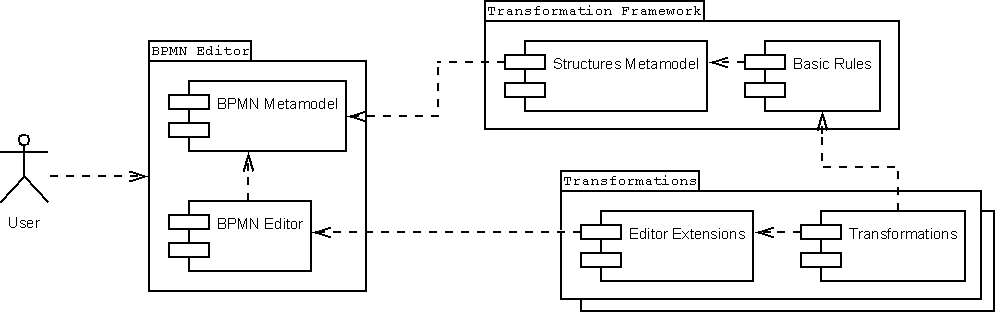
\includegraphics[width=.5\textwidth]{img/vsdt_comp.png}
%	\caption{Architecture of the Visual Service Design Tool.}
%	\label{fig:comp}
%\end{figure}

\subsection{The Metamodel}
\label{sec:editor_meta}

% Ueber die BPMN Spezifikation
The BPMN specification~\cite{omg2006business} describes in detail how the several nodes and connections constituting a BPMN diagram have to look, in which context they may be used and what attributes they have to provide.  However, it does neither give a formal definition of the syntax to be used for the metamodel, nor an interchange format, e.g.\ using an XML Schema Definition (XSD).  Thus the editor's metamodel had to be derived from the informal descriptions in the specification.
% Detaillierte Umsetzung der Spezifikation im Modell
As it was our main concern to keep as close to the specification as possible, we decided not to reuse the existing Eclipse STP BPMN Editor, which uses a simplified model of BPMN.\footnote{\url{http://www.eclipse.org/stp/bpmn/}}  Instead, almost every attribute and each constraint given in the specification has been incorporated into the metamodel, allowing the creation of any legal business process diagram.
% Sachen, wo sich das Modell von der Spezifikation unterscheidet
Still, some attributes have not been adopted in the metamodel:  For instance the possibility to model nested or even crossing Lanes has been dropped, as it turned out that this feature seems to be virtually never used in practical business process design.  Further, redundant attributes, such as the Gateway's \texttt{defaultGate} attribute, are emulated using getter methods to prevent inconsistency in the diagram model.

% StructuredBPMN-Metamodell
Concerning the transformation to BPEL and other executable languages, which in most cases are block-oriented, an extension to the usual BPMN metamodel has been designed, featuring equivalents to the basic block structures, such as sequences, decisions, parallel blocks and loops.  These elements are described in a separate metamodel, extending the editor's metamodel.  They are used only during the transformation process, especially for the mapping of the structure, as we will see in Section~\ref{sec:trafo}.


\subsection{The BPMN Editor}
\label{sec:editor_editor}

% Basis: Eclipse GMF -> Viele gute Features frei Haus
Like many others, the VSDT editor has been created using the Eclipse Graphical Modelling Framework (GMF), automatically equipping the editor with numerous features, such as support for the Eclipse properties, outline and problem view and unlimited undo and redo, just to name a few.  Being embedded in the Eclipse workbench, the editor is easy to use while at the same time providing a powerful tool for professional business architects and service developers.

% Erweiterungen: Property Sheets, Dialoge, Validierung, etc.
While GMF provides a solid basis for the editor, several customisations have been made to the code, further improving the editor's overall usability and supporting the creation of new business processes.  For example, the generated property tables have been supplemented with custom-made sheets, in which the several attributes are more clearly arranged.  For managing the non-visual elements given in the BPMN specification, such as Properties, Messages and Assignments, a number of clear and uniform dialogs has been created.  The various constraints given in the specification were translated to several audit constraints used to validate a given business process diagram.  A screenshot showing some of the editor's features can be seen in Figure~\ref{fig:screen}.

\begin{figure}%[htbp]
	\centering
	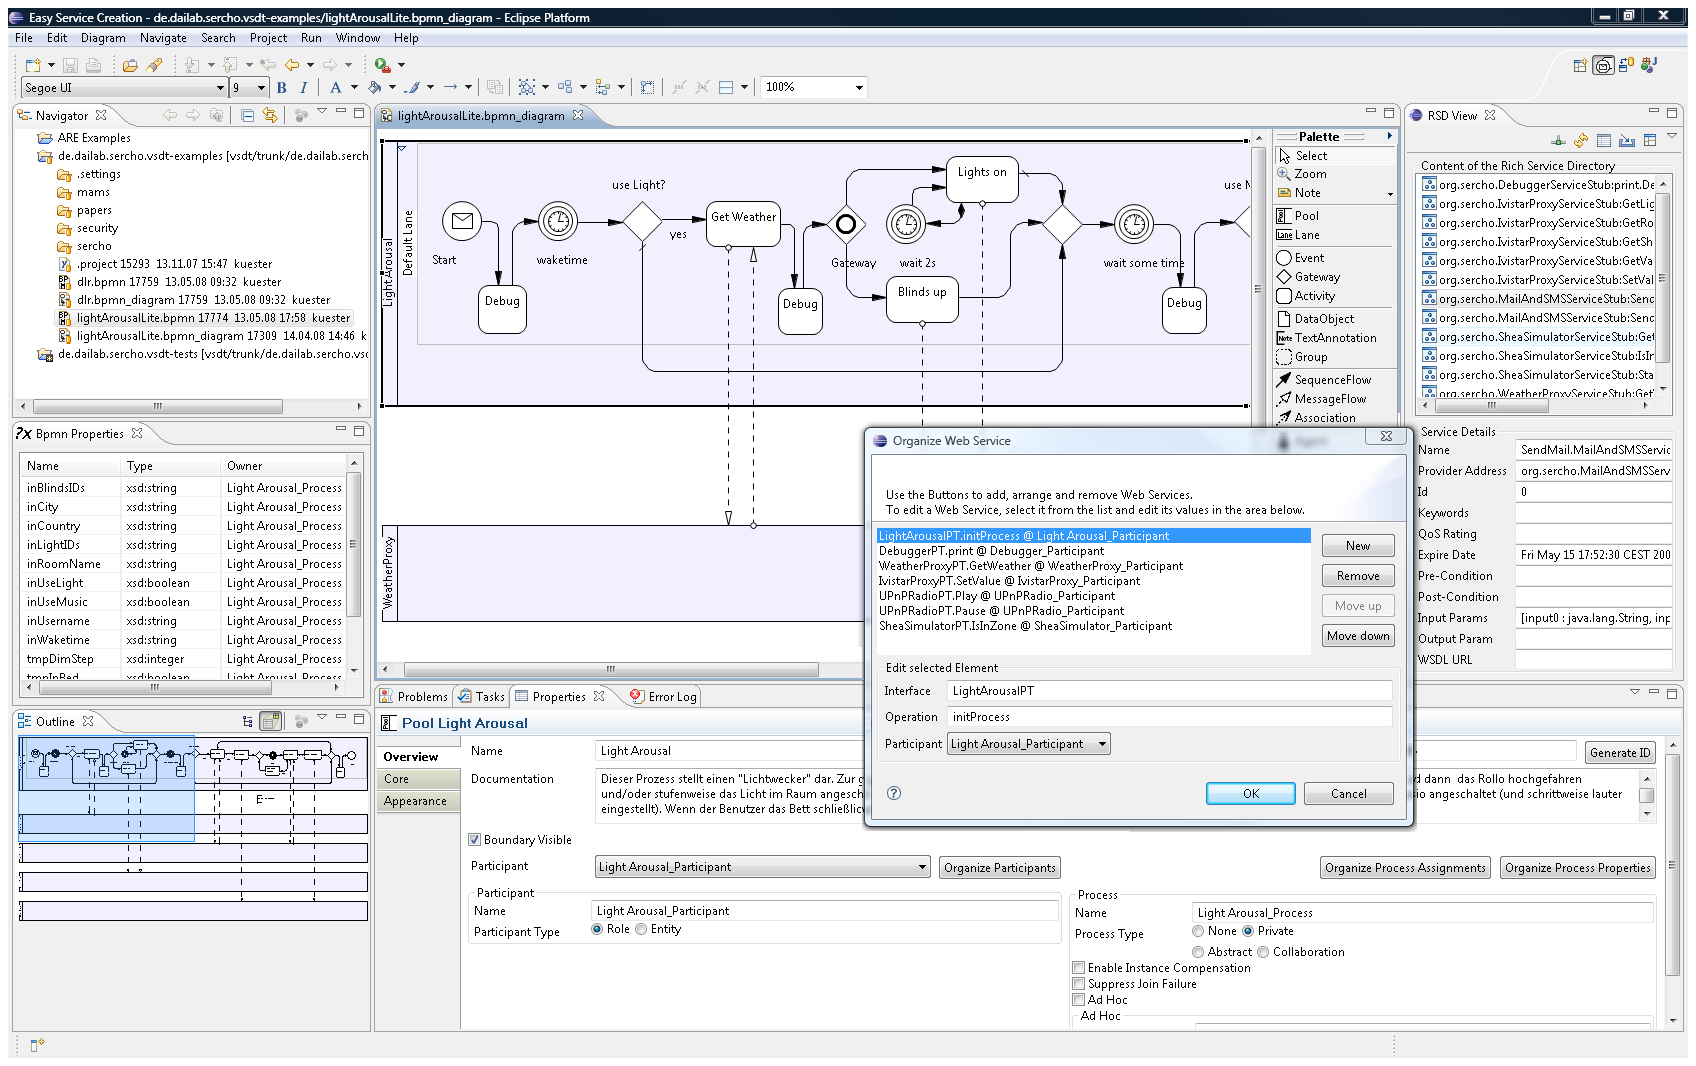
\includegraphics[width=\textwidth]{img/vsdt_080515.png}
	\caption{The Visual Service Design Tool. Clockwise: Editor view, RSD client, web services dialog, property sheet, visual outline, properties inspector, navigator.}
	\label{fig:screen}
\end{figure}

% Nachteil der Erweiterbarkeit/ BPEL-unabhaengigkeit: keine BPEL-Untertuetzung im Editor
As already mentioned, the VSDT was designed to be a pure BPMN editor and independent of BPEL, so the business process diagrams can be transformed to other languages, too, given the respective export plugins. Of course, the downside of this approach is that the editor lacks built-in support for BPEL, e.g.\ the editor itself does not validate an expression given in the diagram to conform to the BPEL syntax.  However, it is possible to supplement the editor with additional plugins, which can contribute e.g.\ to the property sheets or provide whole new views with language-specific functionality.

% Rich Service Directory
One example of how the VSDT can be extended with features specific to a certain target language --- in this case: BPEL --- is the RSD View, which can bee seen in Figure~\ref{fig:screen}, too: A client for the \emph{Rich Service Directory}, a special kind of Web service repository. Using the RSD View, existing Web services that have been registered at the RSD server can be inspected and imported into the diagram.  In the process, an Implementation object is created for the Web service as well as a set of Message objects, matching the service's input parameters and result. Optionally, also a new Pool will be created for the service, which can be connected to the currently selected Activity via a pair of Message Flows.  Further, the Implementation and the Message objects will be associated to the Activity and its type will be set to \textsc{service}.  Thus, the orchestration of existing Web services in a BPEL process can be simplified greatly.  Similar features can be created for other target languages, too.

% Export Wizards
Once the business process diagram is completed it can be validated and exported.  As the VSDT is intended to provide export features to arbitrary target languages, and to support the tool smiths in the creation of these features, we have created an elaborate export framework, which we will have a closer look at in the next section.

\section{The Transformation Framework}
\label{sec:trafo}

The core of the Visual Service Design Tool clearly is the transformation to executable code.  While by now the transformation to BPEL is the only one that can be conveniently used in practice, and thus will serve as an example later in this section, there are currently several other transformations under development.

The transformation framework has been designed from the very beginning to be as \emph{extensible} and \emph{reusable} as possible.  For that purpose the process of transformation has been subdivided into several stages, which are sequentially applied to the input model:
\begin{enumerate}
	\item \emph{Validation}: Validate the input model.
	\item \emph{Normalisation}: Prepare the input model for transformation.
	\item \emph{Structure Mapping}: Convert the input model to a block-like structure.
	\item \emph{Element Mapping}: Perform the actual mapping, create target model.
	\item \emph{Clean Up}: Remove redundancies, improve readability, etc.
\end{enumerate}

% Implementierungsdetails...
%The basic architecture can be seen in Figure~\ref{fig:trafo_framework}.  
The several stages are realised either as a set of graph transformation rules, a top-down pass through the input model, or a combination of both.  For the graph transformation rules the \emph{Tiger EMF Model Transformation} Framework~\cite{biermann2006graphica} (EMT) has been employed, providing a fast pattern matching and backtracking algorithm for EMF models.  In EMT, rules can be specified using a convenient graphical editor.  For the VSDT, however, the EMT has been modified so that instead of a Left Hand Side (LHS) with Negative Application Conditions (NACs) and a Right Hand Side (RHS), the rules feature an LHS, NACs and an \texttt{execute} method, which may contain arbitrary Java code.  Given the several cases to consider in BPMN this has proven more feasible.  The transformation is operating on a copy of the model to be transformed, which can be modified in the course of the transformation without affecting the original diagram.

%\begin{figure}%[htbp]
%	\centering
%	\includegraphics[width=\textwidth]{img/trafo_framework.png}
%	\caption{Essential classes of the transformation framework, including the BPEL case.}
%	\label{fig:trafo_framework}
%\end{figure}

\subsection{Stages of the Transformation}
\label{sec:trafo_stages}

%  Zielsprachen-Unabhaengigkeit von Validation, Normalisation und Structure Mapping
The Validation, Normalisation and Structure Mapping are to a great part independent of a specific target language, and in most cases the standard implementations provided with the transformation framework can be used.  However, it can be advantageous to extend them with additional checks and rules.

% Validation
For instance, in the \emph{Validation} stage, all identifiers are validated to contain only characters that are legal with respect to the given target language, which can be achieved by extending the standard implementation and using a respective regular expression for the validation of names.  Further, the validation includes a pass through the model, checking if each element needed is in place, thus reducing the number of checks necessary in the actual transformation, and providing clearer error messages to the user in case something is missing.

% Normalisation
The intent of the \emph{Normalisation} stage is to put the process diagram in a uniform form, and to transform it to what in the following will be referred to as the BPD's \emph{normal form}, a semantically equivalent representation of the diagram following more strict constraints than those given in the BPMN specification.  The transformation rules that are used in this stage are rather simple.  For instance, one rule will check if there are any Activities with multiple incoming or outgoing Sequence Flows attached to it, in which case a Gateway of type \textsc{xor} or \textsc{and}, depending on whether the Sequence Flows have any conditions, will be inserted in between.  Another rule will insert a ``no-op'' Activity in between any two Gateways that are directly connected by a Sequence Flow.  The advantage is that after the application of the normalisation stage there will be much fewer cases to consider in the structure mapping, which will be described in the next paragraph. A simple example of the consecutive execution of normalisation and structure mapping can be seen in Figure~\ref{fig:norm_struc}.

\begin{figure}%[htbp]
	\centering
	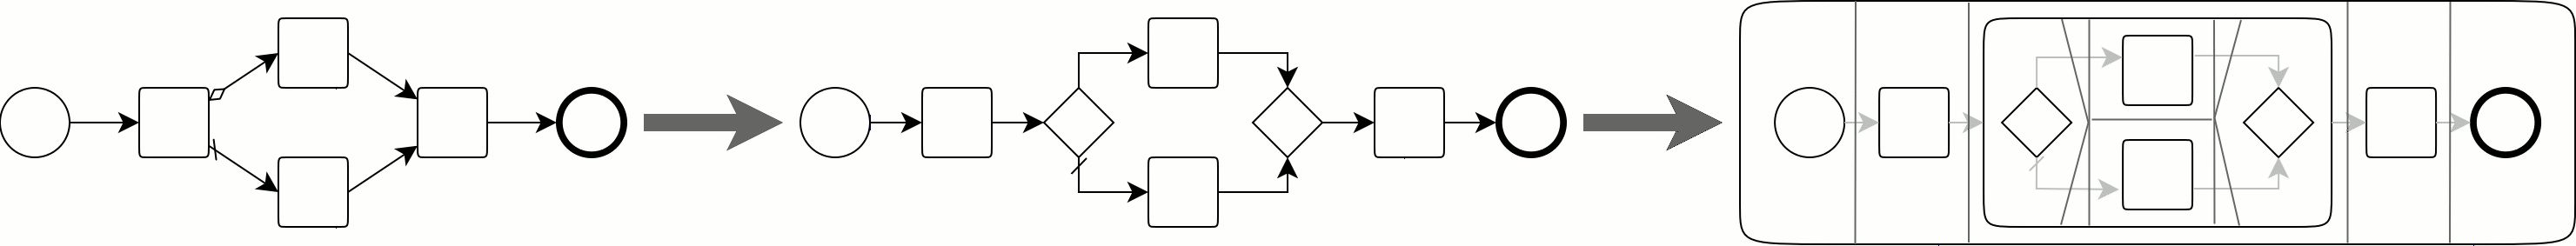
\includegraphics[width=\textwidth]{img/norm_struc_2.png}
	\caption{Simple example of normalisation and structure mapping.}
	\label{fig:norm_struc}
\end{figure}

% Structure Mapping
One of the challenges in transforming BPMN to executable languages is the mapping of the process model's graph-oriented structure to a more rigid block-oriented structure.  For that reason it is of great benefit making this part, the \emph{Structure Mapping}, independent of the actual target language, so it can be reused in mappings to other block-oriented languages.  We decided to follow a \emph{Structure Identification} strategy~\cite{mendling2005transformation}, being independent of BPEL's Link element.  As mentioned in Section~\ref{sec:editor_meta}, the transformation is using an extension of the BPMN metamodel used in the editor, allowing the introduction of additional elements representing sequences, blocks for parallel and alternative routing, loops, and event handler blocks, i.e.\ the basic building blocks of block-oriented languages.  Now, in the structure mapping stage, the model is searched for graph patterns which are semantically equivalent to these blocks, e.g.\ two Flow Object nodes connected with a Sequence Flow, or two Gateways connected by a number of branches of Flow Objects.  When such a pattern is found, it is replaced with the respective structured element, removing the involved Sequence Flow edges in the course, which are then no longer needed (their conditions, if any, are preserved in the newly created structured elements).  With these elements themselves being Flow Objects again, the rules of the structure mapping are applied until the entire process within each Pool has been reduced to a single complex element, e.g.\ a sequence, or until it can not be reduced any further due to structural flaws.  Some examples of BPMN graphs that can successfully be mapped to equivalent block structures and further to executable BPEL code can be seen in Figure~\ref{fig:structures}.  Of course, this stage can be adapted or entirely omitted, too, if the target language is structured differently.

\begin{figure}%[htbp]
	\centering
	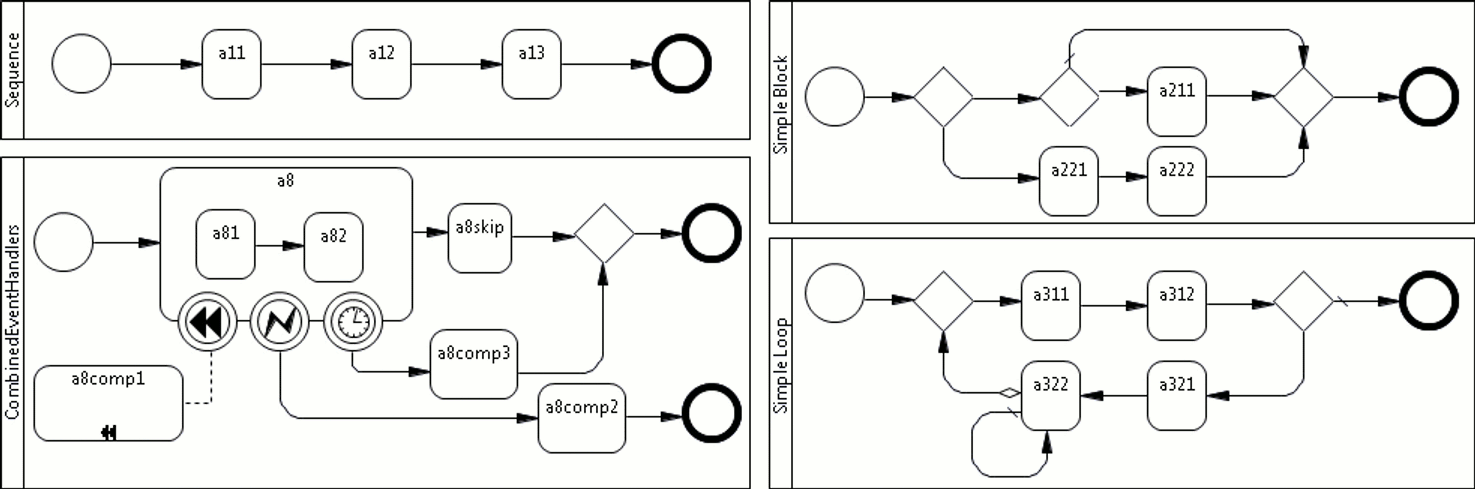
\includegraphics[width=\textwidth]{img/structures.png}
	\caption{Some examples of transformable BPMN graphs.}
	\label{fig:structures}
\end{figure}

% Element Mapping
After the rule-based structure mapping, in the \emph{Element Mapping} stage, the several BPMN elements can be mapped in a relatively simple top-down pass through the model.  We decided to use a top-down pass instead of rules in this stage, as it is faster and easier to maintain, but the framework does allow for other implementations as well.  As the element mapping is very dependent on the actual target language we will go further into detail later, regarding the transformation to BPEL.

% Clean Up
Finally, in the \emph{Clean Up} stage, a set of rules is applied on the newly created target model.  While this stage is optional, it can be of great use for improving the readability of the generated code while at the same time keeping the required logic out of the earlier stages.  For instance, nested sequences will be flattened, or sequences that hold a single element are replaced by that element itself.  Further, elements that resulted from no-op Activities inserted in the normalisation stage should be removed again in this stage.  As this stage operates on the target model, is has to be implemented anew for each target language.

For implementing a specific transformation, all that has to be done is to specify the element mapping, which can be done in any desired fashion by extending a special abstract class (see Figure~\ref{fig:trafo_framework}). In case the target language uses different block concepts, the structure mapping has to be adapted, too, but should still be reusable to some point.  In the majority of cases, implementing the other stages is optional.

\begin{figure}%[htbp]
	\centering
	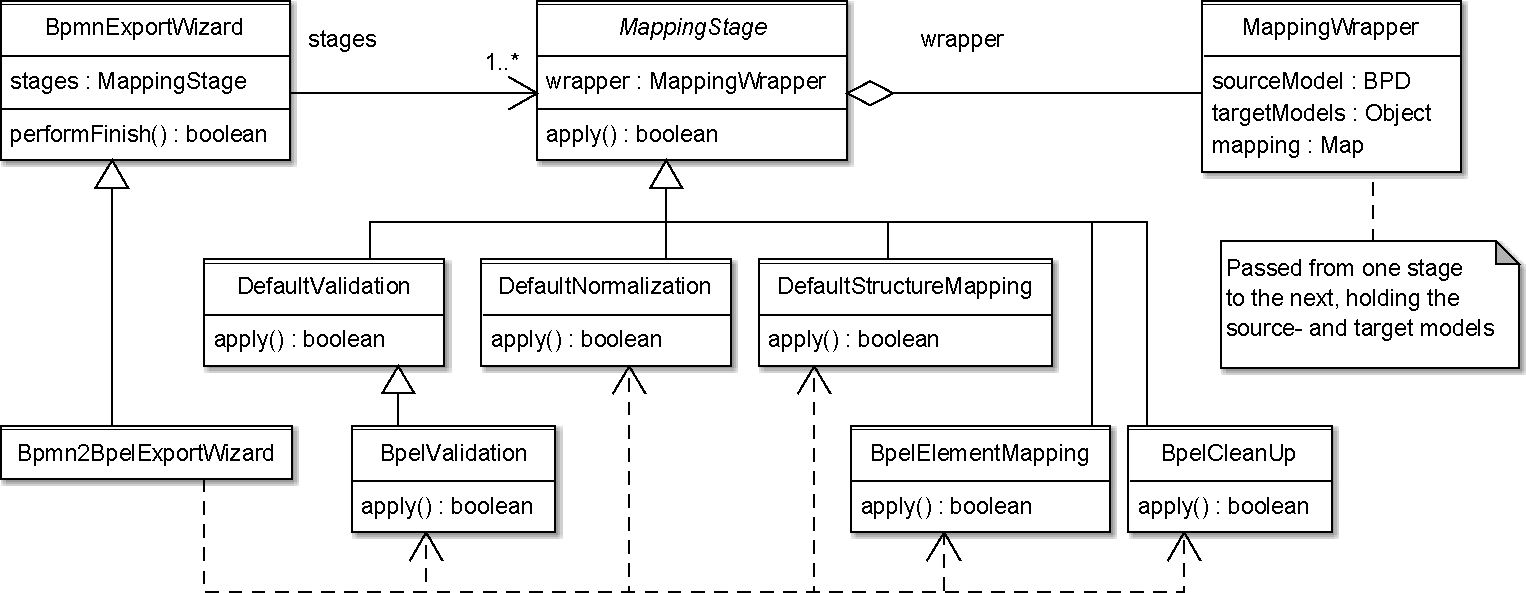
\includegraphics[width=\textwidth]{img/trafoframework.png}
	\caption{Essential classes of the transformation framework, including the BPEL case.}
	\label{fig:trafo_framework}
\end{figure}


\subsection{Transformation to BPEL}
\label{sec:trafo_bpel}

The transformation to BPEL presented in this work covers nearly the entire mapping as given in the BPMN specification~\cite[Chapter 11]{omg2006business}, including event handlers, inclusive \textsc{or} and event-based \textsc{xor} Gateways, just to name a few.  Still there are some elements for which the mapping is not given very clearly, such as \textsc{timer} Start Events, independent Sub Processes or multi-instance parallel loops.  While these elements will be transformed as described in the specification, the resulting BPEL processes will require some amount of manual refinement.  Besides the BPEL process files a WSDL definitions file is created, holding the message types derived from the process properties and the input and output messages and interfaces (port types) for the several Web services being orchestrated by the process.  Still, the WSDL's binding and service blocks and necessary schema types, if any, can not be generated automatically yet, due to insufficient information in the source model.  We are currently investigating ways of extending the BPMN metamodel in order to include more information in the model and at the same time making it more independent of the BPEL language.

In the validation used for the transformation to BPEL, all identifiers are tested to contain only characters that are legal with respect to BPEL.  Additionally all expressions used e.g.\ in Assignments and loop conditions are scanned for occurrences of Property identifiers.  So if a Process \texttt{Proc} has a Property \texttt{foo} and there is an Assignment with an expression like \texttt{"foo+1"}, the expression will be changed to \texttt{"bpws:getVariableData('Proc\_ProcessData','foo')+1"}.  Thus the user does not have to care about the way Properties are represented with messages in BPEL but can use a Property's plain name in expressions.


\subsection{Example}
\label{sec:trafo_example}

The following example will show one of the scenarios being used in a smart home environment in the SerCHo project.  The resulting BPEL processes were validated and tested with the \emph{ActiveBPEL} designer and process engine.\footnote{\url{http://www.activebpel.org}}

The BPMN diagram in Figure~\ref{fig:example} is showing a ``Light Alarm'' process, that is used to open the blinds in the user's room to wake her up in a more pleasant way than the usual alarm clocks do.  For that purpose, firstly information on the current weather is retrieved using an external Web service.  Thereafter, based on the weather data, either the sunblinds are opened, or the ceiling light is turned on, or both.  In case the user does not get up, which is checked using an RFID based localisation solution, the stereo is turned on, playing her favourite song or alternatively an unpleasant alarm sound.

\begin{figure}%[htbp]
	\centering
	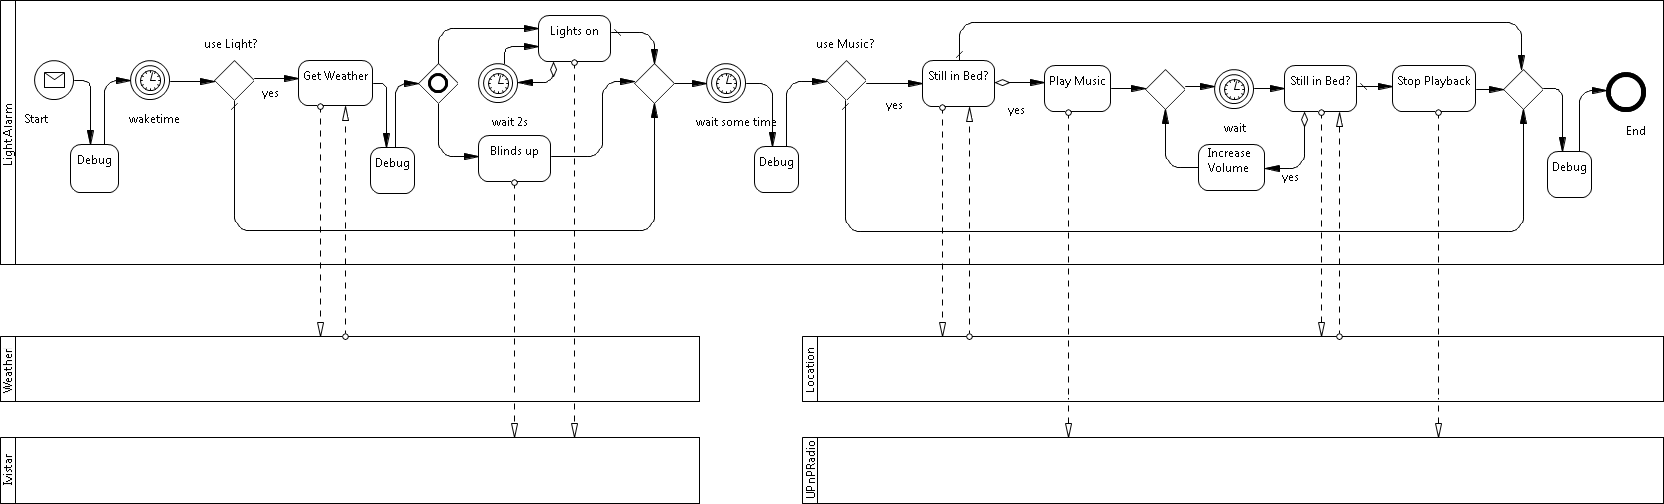
\includegraphics[width=\textwidth]{img/demo_lichtwecker_kompakt.png}
	\caption{``Light Alarm'' Example Process}
	\label{fig:example}
\end{figure}

For each of the above devices --- blinds, lights, localisation, and stereo --- Web service interfaces were written, so they can be integrated in a BPEL process.  While the WSDL file that is used by the process, holding the definitions for the various orchestrated services, has to be extended with the service bindings, the BPEL code resulting from this example is readily executable.


\subsection{Transformation to JIAC}
\label{sec:trafo_jiac}

Concerning our goal of transforming BPMN diagrams to multi-agent systems (MAS) the work is still at an early stage.  First, a \emph{normal form} for BPMN diagrams has been investigated, to facilitate the mapping~\cite{endert2007towards}.  Later, the first steps of the actual mapping have been developed, basically mapping Pools to agents, Processes and Flow Objects to the agents' plans and the control flow, and Message Flow to the exchange of messages between the agents~\cite{endert2007mapping}.

A first prototype targeting the agent framework JIAC IV~\cite{sesseler2002modularearchitektur} has already been implemented.  As the theoretical part of the mapping is not yet fully matured, there is still some work to do.  However, with the given transformation framework every addition to the mapping can quickly be adopted.


\section{Related Work}
\label{sec:sota}

% grosse zahl von BPMN-Editoren, die meisten nur Zeichen-Tools ohne Export
The Business Process Modelling Notation has been adopted in a large number of tools.  Although many of these are merely diagram drawing tools and do not support the transformation to BPEL, let alone other languages, there are some powerful tools as well.  In the following we will introduce some of these.  A more extensive list can be found at \url{http://www.bpmn.org/BPMN_Supporters.htm}.

% Soyatec eBPMN und Eclarus SOA Architect
With the free \emph{eBPMN}, Soyatec provides a very nice BPMN editor, but it does not implement the mapping to BPEL.\footnote{\url{http://www.soyatec.com/ebpmn}}  The same applies to the free community edition of eClarus' \emph{Business Process Modeller}, while the commercial \emph{SOA-Architect} version provides a transformation to BPEL, although it seems to have some limitations.\footnote{\url{http://www.eclarus.com/}}
% Intalio / Eclipse STP
A very mature BPM product can be found in the \emph{Intalio BPMS}.\footnote{\url{http://www.intalio.com/}}  BPEL code is generated on-the-fly and can be deployed to the Intalio process engine.  However, the mapping of workflow structures is limited, e.g.\ we found it impossible to merge a branch originating from an event handler back into the normal flow.  Another limitation arises from the tight coupling to the in-house BPEL engine, which is using some proprietary extensions.  Further, Intalio has donated parts of the code to the Eclipse SOA Tools Project (STP).  While the \emph{STP BPMN Editor} itself does not provide a transformation to BPEL, Giner et.al.\ were able to combine it with the \emph{BABEL Bpmn2Bpel} tool~\cite{giner2007bridging}, yet both the editor and the transformation tool are using very simple metamodels.


% Mapping von Unstructured Workflows
Concerning the transformation from graph-oriented to block-oriented process models, as in the BPMN to BPEL case, Mendling et.~al.\ have evaluated several transformation strategies~\cite{mendling2005transformation}, ranging from a straight-forward mapping of BPMN Sequence Flows to BPEL Links, similar to the one in~\cite{white2005using}, to a more sophisticated \emph{Structure Identification} strategy, like the one applied in this work, or \emph{Structure Maximisation}, as followed by Aalst and Lassen~\cite{aalst2008translating}.  In their theoretically well-founded, pattern-based transformation from Petri nets to BPEL, they focus on the readability of the resulting code.  However, they do not regard how highly \emph{unstructured} workflows can be transformed to structured ones.  As pointed out in~\cite{recker2006translation}, there is a ``mismatch'' between BPMN and BPEL, both on the domain representation and the control flow level, that is not easily to overcome.  Many authors have investigated whether different graph patterns can be transformed to an equivalent structured form~\cite{Kiepuszewski2000structured, liu2005Analysis, sadiq2000analyzing}, and came to the conclusion that even slight unstructuredness can require the introduction of additional variables or the duplication of parts of the workflow, even though the workflow models used in these works are much simpler than BPMN.  For structuring such workflows, Koehler et.~al.\ present a rule-based transformation based on continuation semantics~\cite{koehler2004untangling}.  Another approach is followed by Ouyang et.~al., using BPEL event handlers as a form of \texttt{goto} command~\cite{ouyang2006translating_standard}.  Their examples show how complicated a simple workflow can become when being structured.

Thus, as workflow design will be facilitated greatly if the user is not restricted to the use of block-oriented processes, a transformation of unstructured workflows to readily executable code will be highly desirable, so that such processes can be created by means of Model Driven Engineering.

\section{Conclusion}
\label{sec:conclusion}

% BPMN->BPEL, erweiterbar, Trafos und Editor-Features reinpluggen
In this paper the \emph{Visual Service Design Tool} (VSDT) has been introduced: a BPMN editor featuring a state of the art transformation to BPEL, while at the same time being easily extensible with export functionality targeting other languages.  The editor itself has been designed to be language independent, so it can be used for generating code for any language, given that a respective mapping from BPMN to that language exists.
% Trafo-Framework
Transformations implementing these mappings can be plugged in to the VSDT together with additional editing features helping the user in the creation of diagrams to be exported to that language.  For supporting the developer of these plugins, the VSDT comes with a transformation framework, based on the EMT graph transformation tool.  Being subdivided into several stages, large parts of it can be reused throughout different mappings, such as the refactoring of the process graph to block-oriented structures.

% Dieser Teil ueber die Trafo nach BPEL
With respect to its BPMN editing functionality and the transformation to BPEL, the VSDT does not have to hide behind its commercial competitors.  Implementing the mapping to BPEL as given in the BPMN specification, the tool can be used to generate readily executable code.  Still it is recommended to validate the results with a native BPEL editor:  While the creation of processes will be easier and faster using the VSDT, its desired independence of a specific language prohibits some BPEL specific features, such as editing assistance for assignment expressions.  However, due to the plugin architecture provided by the Eclipse platform, such functionality can be added together with the actual transformation features.

As the key feature of the VSDT is the extensibility with additional export features, further transformations from BPMN to executable languages are currently under development.  One of the main goals of our research in this field is a mapping from BPMN to multi-agent systems, combining the intuitive design of business processes with the flexibility of software agent.


\subsection{Future Work}
\label{sec:conc_future}

Some work still can be done in the field of transformation of unstructured processes.  Currently the tool can handle slightly unstructured workflows, such as one Gateway being used for merging multiple decision blocks, but will fail when faced with e.g.\ overlapping blocks or multiple exits from a loop.  Here, further evaluations of the different possibilities to handle such workflows and ways of adapting them to the more complex BPMN diagrams will be necessary.

Concerning the transformation to BPEL, the support for complex data types will need further refinement.  Here, the \emph{Rich Service Directory} introduced earlier will be of great use, providing the necessary information about the involved Web services.  Finally, the mapping to multi-agent systems has to be completed, and mappings to further languages will be evaluated.


\bibliographystyle{plain}
\bibliography{act-db}

\end{document}
